
\chapter{Quantization Step Size Selection}\label{chap:deltaq}

The selection of a time step ($\Delta t$) for a time-slicing simulation method usually involves a straight-forward trade-off between accuracy and performance. For time-slicing, the smaller the $\Delta t$, the more accurate the results (with a lower bound on $\Delta t$ for numerical stability). One might assume that the same straight-forward trade-off exists between accuracy and performance when selecting the quantization step size ($\Delta Q$) for a QSS-based simulation. After all, there is a direct relationship between $\Delta Q$ and the amount of elapsed time before the next update will need to be updated. For a first-order QSS integrator of a single state variable, this is a simple relationship of $\Delta t = \Delta Q \cdot d$, where $d$ is the current derivative of the state. of  However, although it is generally true that lower $\Delta Q$ tends to result in more computational load and higher simulation accuracy, the relationship is complicated. 

To illustrate this, the performance of the synchronous machine simulation from chapter \ref{chap:syncmach} is repeated here in figure \ref{fig:syncmach_error_qstep_all_2}, and shows the error and computational load of the synchronous machine simulation as a function of $\Delta Q$. In this simulation, all flux and speed states of the machine have the same $\Delta Q$ for each simulation run, with the exception that the machine rotor angle is scaled to be $1/10^{th}$ of the $\Delta Q$ of the the other states to account for the finer resolution needed due to a significantly lower dynamic range of this state. The error quantity is the largest normalized time-averaged error relative to reference ODE simulation (the maximum normalized root mean squared deviation, or NRMSD, among all system states). Although the error generally increases with an increasing quantization step size (as expected), the relationship is non-linear, sporadic at higher $\Delta Q$ values, and shows significant diminishing returns at lower $\Delta Q$ values. These results, and those from other simulations performed in this document, show that the selection of optimal (or even \emph{suitable}) $\Delta Q$ values for a simulation is not a straight-forward process.

\begin{figure}[h]
    \centering
    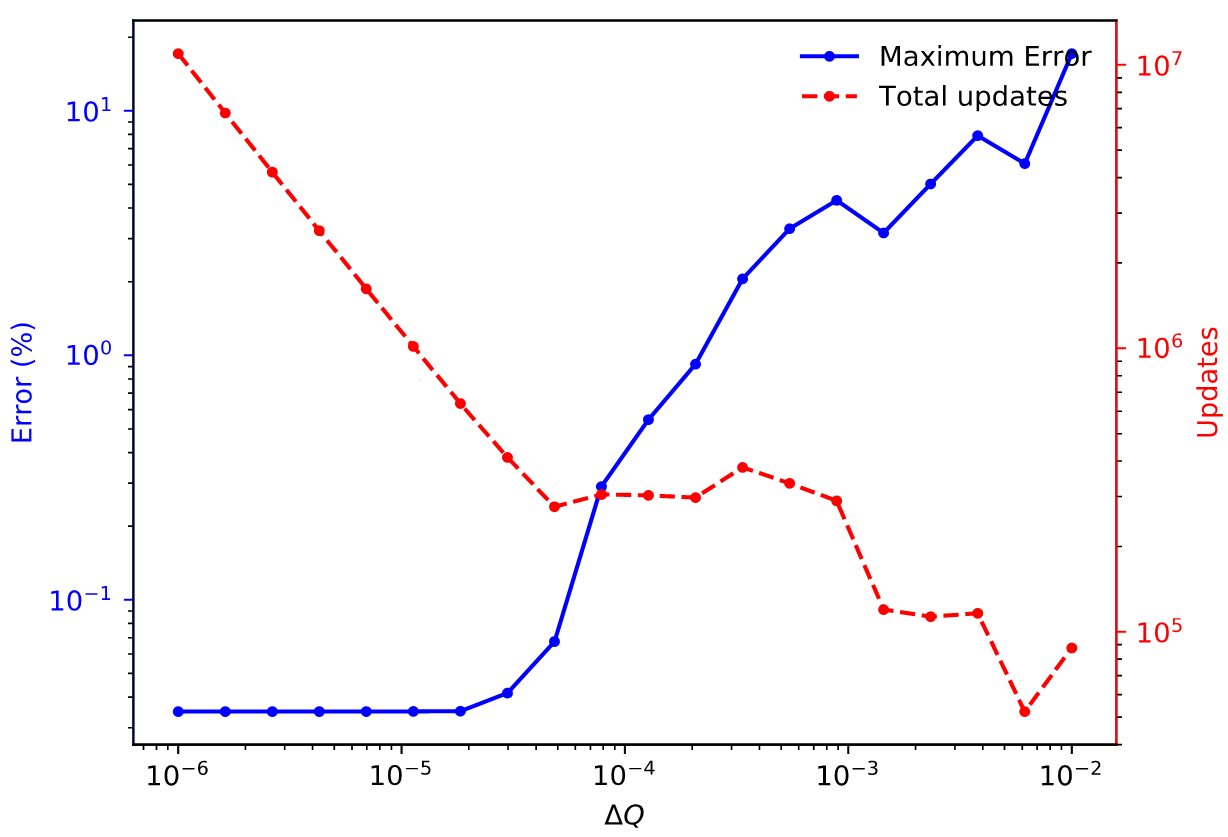
\includegraphics[width=0.8\linewidth]{syncmach_error_qstep_all.png}
    \caption{Maximum Error (among all system states) and QDL updates for various base values of $\Delta Q$ from the synchronous machine system simulation from chapter \ref{chap:syncmach}.}
    \label{fig:syncmach_error_qstep_all_2}
\end{figure} 


The selection of $\Delta Q$ is also complicated by the fact that each QDL atom in general needs its own $\Delta Q$ value for optimal simulation performance and suitability of the results. This can be clearly understood by considering the case of a system that contains a per unit PID controller model, along with a Megawatt level electrical load. The controller states may require quantization steps on the order of $10^{-6}$, while the load current states may be quantized with a step on the order of $10^{-1}$. 

Ideally, the engineer should provide the desired acceptable error levels for the outputs of interest in a simulation, and the optimal $\Delta Q$ values for each atom are then automatically determined in order to maximize the quantization step size given the acceptable error constraints, while minimizing the computational load for the simulation. Again, for time-slicing simulation methods, this is typically as simple as setting the time step at large as possible given the stability constraints determined by an eigenvalue analysis, perhaps with a margin added to account for the effects of non-linearity. Several methods for approaching an optimal selection of $\Delta Q$ for a QSS-based methods were attempted.

The initial approach to providing suitable $\Delta Q$ values was to assume that the error of each state is bounded by exactly $+$/$-$ $\Delta Q$, and choose the $\Delta Q$ values accordingly. This has the advantage of being very simple, but the core assumption proved to be very incorrect. Because of the propagation of error that occurs between coupled states, the error levels at any given state can be larger than $\pm \Delta Q$ in general. The next attempt involved setting the $\Delta Q$ based on the dynamic range of each state. For example, each state's $\Delta Q$ can be set equal to 1\% of the known dynamic range of the state variable as determined by a reference traditional ODE simulation result. This provided a good way to test the QDL method, but it has the obvious problem of requiring a solved reference simulation before the QDL simulation can be performed. This is therefore not suitable as a general method for selecting $\Delta Q$. Finally, a method that exploits the signal propagation behavior of the QDL method was developed. This method is described below.

\section{The Error Propagation Method for $\Delta Q$ Selection}

If the Jacobian matrix of he dynamic system can be determined at a given operating point, the linear sensitivities between external state transitions and the internal state of each atom is known. The amount of change possible during a given atom's external state transition can therefore be limited to arbitrary bounds by setting the quantization step size of all connected atoms based on their respective sensitivities. Stated another way: each atom's error is controlled by setting its connected neighbor atoms' quantization steps appropriately. This method uses common uncertainty calculations to attempt to maximize each state's $\Delta Q$ by interpreting uncertainty as a proxy for desired error bounds. 

Given the input variances for a state vector $\mathbf{\sigma^x}$, the output variances $\mathbf{\sigma^y}$ are found using the additive propagation rule

\begin{equation} \label{eq:err_prop}
\sigma_i^y = \sqrt{  \sum_{j=1}^{N}{ \left( \frac{\partial f_i}{\partial x_j} \right) ^2 ( \sigma_j^x)^2 } }
\end{equation}

where $( \partial f_i / \partial x_j )$ is the element of the Jacobian between the $i^{th}$ and $j^{th}$ atoms. We then replace the variance vectors $\mathbf{\sigma^x}$ and $\mathbf{\sigma^y}$ with the quantization step vectors $\Delta Q^y$ and $\Delta Q^x$ as

\begin{equation} \label{eq:err_prop2}
\Delta Q_i^y = \sqrt{  \sum_{j=1}^{N}{ \left( \frac{\partial f_i}{\partial x_j} \right) ^2 (\Delta Q_j^x)^2 } }
\end{equation}

where $\Delta Q_i^y$ is the output quantization step for the $i^{th}$ atom, and $Q_j^x$ is the input quantization step for the $j^{th}$ atom. For our purposes, the output quantization step vector can be interpreted as the desired maximum allowed error in the quantized output (this is the error bound vector), and the input quantization step vector will be calculated in order to honor the desired maximum error (this is the QDL $\Delta Q$ vector). Therefore, the QDL $\Delta Q$ vector can be found by solving for $Q_j^x$. We define the squared quantization step vectors as

\begin{equation} \label{eq:covar_sy}
\mathbf{s^y} = 
\begin{bmatrix}
\left( \Delta Q_1^y \right)^2 &
\left( \Delta Q_2^y \right)^2 & \dots &
\left( \Delta Q_N^y \right)^2
\end{bmatrix}^\top
\end{equation}

\begin{equation} \label{eq:covar_sx}
\mathbf{s^x} = 
\begin{bmatrix}
\left( \Delta Q_1^x \right)^2 &
\left( \Delta Q_2^x \right)^2 & \dots &
\left( \Delta Q_N^x \right)^2
\end{bmatrix}^\top
\end{equation}

and rewrite (\ref{eq:err_prop2}) in matrix form

\begin{equation} \label{eq:solve_for_dq1}
\mathbf{s^y} = \mathbf{ \left( J^\top J \right) s^x }
\end{equation}

and rearrange to solve for $\mathbf{s^x}$ 

\begin{equation} \label{eq:solve_for_dq2}
\mathbf{s^x} = \mathbf{ \left( J^\top J \right)}^{-1} \mathbf{s^y}
\end{equation}

where $\mathbf{J}$ is the full Jacobian matrix of the system. The quantization steps used in the simulator are found as the square root of the elements of $\mathbf{s^x}$

\begin{equation} \label{eq:dq_final}
\mathbf{\Delta Q} = 
\begin{bmatrix}
\sqrt{|s_1^x|} &
\sqrt{|s_2^x|} & \dots &
\sqrt{|s_N^x|}
\end{bmatrix}^\top
\end{equation}

For the linear, time-invariant case, the Jacobian is equal to the state matrix, and does not change throughout the simulation. For the time-varying, non-linear case, however, the Jacobian is a function of time and the current state vector, and using the Jacobian to determine the error propagation is only an approximation. The approximation of $\Delta Q$ can be improved by calculating the Jacobian at the initial and final states when a system perturbation event occurs. The minimum values of $\Delta Q$ can then be used from solving (\ref{eq:solve_for_dq2}) for both $\mathbf{J}_0$ and $\mathbf{J}_\infty$. 

\section{Error Control Example}

An interesting test case is a second-order, non-linear pendulum. It is small enough to keep the analysis simple, but has some features of the non-linear dynamics of complex power systems. For this example, the choice of $\Delta Q$ is intentionally chosen to be large relative to the amplitude of the transients of the simulation so the effects of the error method can be seen clearly.  

The dynamics of a damped pendulum are described by the second order system

\begin{equation} \label{eq:pendulum1}
\frac{d^2}{dt^2} \theta = -r \frac{d}{dt} \theta -\frac{g}{l} \sin{\theta}.
\end{equation}

Which can be rewritten as two first-order equations as

\begin{equation} \label{eq:pendulum_omega}
\frac{d}{dt} \omega = -r \omega - \frac{g}{l} \sin{\theta},
\end{equation}

\begin{equation} \label{eq:pendulum_theta}
\frac{d}{dt} \theta = \omega.
\end{equation}

Linearizing about the operating point $( \omega_0, \theta_0 )$, the system can be rewritten in the linear form

\begin{equation} \label{eq:pendulum_linearize}
\frac{d}{dt} \mathbf{x} = \mathbf{J} \cdot \mathbf{x} 
\end{equation}

where $\mathbf{x}$ is the state vector $\begin{bmatrix} \omega & \theta \end{bmatrix}^\top$ and $\mathbf{J}$  is the Jacobian matrix

\begin{equation} \label{eq:pendulum_jac}
\begin{bmatrix}
-r & -\frac{g}{l} \cos{\theta} \\
1 & 0
\end{bmatrix}.
\end{equation}

The desired error for the QDL simulation is

\begin{equation} \label{eq:pendulum_dqy}
\mathbf{\Delta Q^y} =
\begin{bmatrix}
0.2 \,\text{rad/s} & 0.4 \,\text{rad}
\end{bmatrix}^\top
\end{equation}

Using $\Delta Q^y$ directly as the $\Delta Q$ vector for the QDL simulation results in a $\theta$ trajectory that deviates significantly outside of the desired error bounds, while the trajectory of $\omega$ remains within bounds at steady state, while deviating only slightly outside of the bounds during the transient figure \ref{fig:pendulum_1}.

\begin{figure}[h]
    \label{fig:pendulum_1}
    \centering
    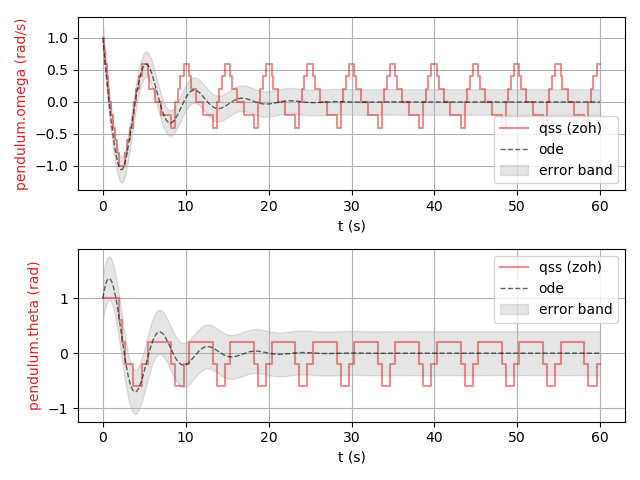
\includegraphics[width=0.8\linewidth]{pendulum_1.png}
    \caption{QDL pendulum simulation results with $\Delta Q_\omega = 0.2$ and $\Delta Q_\theta = 0.4$}
\end{figure}

To apply the selection process from (\ref{eq:solve_for_dq2}), we need to find two Jacobian matrices, one for the initial state of $\begin{bmatrix} 1 \,\text{rad/s} & 1 \,\text{rad} \end{bmatrix}$, which is 
 
\begin{equation} \label{eq:pendulum_jac1}
\mathbf{J}_{0} =
\begin{bmatrix}
-0.4 & -0.6626 \\
1 & 0
\end{bmatrix}
\end{equation},

and another for the final equilibrium state of the $\begin{bmatrix} 0\,\text{rad/s} & 0\,\text{rad} \end{bmatrix}$

\begin{equation} \label{eq:pendulum_jac2}
\mathbf{J}_{\infty} =
\begin{bmatrix}
-0.4 & -1.2263 \\
1 & 0
\end{bmatrix}
\end{equation}.

Note that the equilibrium state of the damped, non-forced pendulum system is defined as $\begin{bmatrix} 0\,\text{rad/s} & 0\,\text{rad} \end{bmatrix}$. In general, finding $\mathbf{J}_{\infty}$ at the final equilibrium point post-disturbance requires solving the non-linear system using a Newton-Raphson solution or some other iterative approach.

From $\mathbf{J}_{0}$ and $\mathbf{J}_{\infty}$ we use (\ref{eq:solve_for_dq2}) to obtain the two $\Delta Q^x$ vectors

\begin{equation} \label{eq:pendulum_dq1}
\mathbf{\Delta Q^x_{0}} =
\begin{bmatrix}
\ 0.4 \,\text{rad/s} & 0.1811 \,\text{rad} \\
\end{bmatrix}^\top
\end{equation}

\begin{equation} \label{eq:pendulum_dq2}
\mathbf{\Delta Q^x_{\infty}} =
\begin{bmatrix}
\ 0.4 \,\text{rad/s} & 0.0979 \,\text{rad} \\
\end{bmatrix}^\top
\end{equation}.

Taking the minimum values from the elements of these two candidate quantization step vectors, the final $\mathbf{\Delta Q}$ vector used for the  QDL simulation is

\begin{equation} \label{eq:pendulum_dq_final}
\mathbf{\Delta Q} =
\begin{bmatrix}
\ 0.4 \,\text{rad/s} & 0.0979 \,\text{rad} \\
\end{bmatrix}^\top
\end{equation}

An important feature of this method is that the resultant $\mathbf{\Delta Q}$ vector can have elements larger than the error vector $\mathbf{\Delta Q^y}$.

The simulation results with the new $\mathbf{\Delta Q}$ is shown in figure \ref{fig:pendulum_2}, where the amplitude of the steady-state oscillations remain bounded within the desired error band (denoted with the gray filled area around the ODE curve). 

\begin{figure}[h]
    \label{fig:pendulum_2}
    \centering
    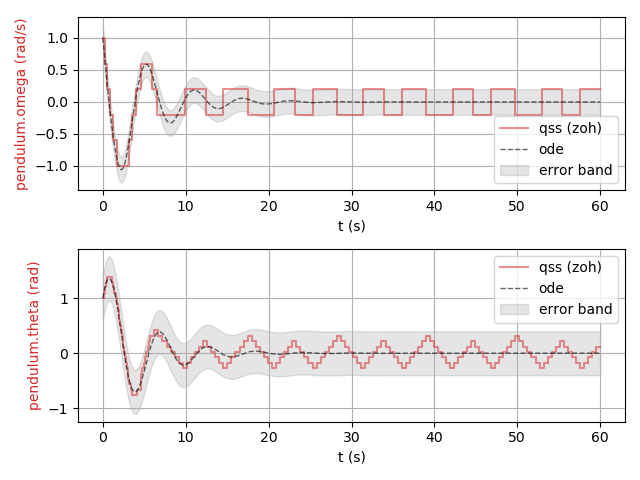
\includegraphics[width=0.8\linewidth]{pendulum_2.png}
    \caption{QDL pendulum simulation results with $\Delta Q_\omega = 0.05$ and $\Delta Q_\theta = 0.1$}
\end{figure}

Note that, although the external state trajectories of both system states plotted in figure \ref{fig:pendulum_2} remain bounded within the desired error band, there is still significant movement about an average values in the nominally steady-state portion of the simulation. Because the error bounds were selected to be large for this simulation to amplify the performance of the $\Delta Q$ selection method, the oscillations typical of the QDL steady-state results are easy seen. This behavior often takes the form of an apparent limit cycle, sometimes with a clear period. The hypotheses is that this perpetuated limit cycle behavior is an artifact of the QDL method caused by fictitious energy injection arising from the difference between the internal state values and their propagated quantized states. This phenomenon, along some potential mitigation methods, are explored in the following chapter.
